\documentclass[dcc,uchile]{fcfmcourse}
\usepackage{teoria}
\usepackage[utf8x]{inputenc}
\usepackage{amsmath}
\usepackage{amsfonts,setspace}
\usepackage{listings}
\usepackage{hyperref}
\usepackage{color}





\definecolor{pblue}{rgb}{0.13,0.13,1}
\definecolor{pgreen}{rgb}{0,0.5,0}
\definecolor{porange}{rgb}{0.9,0.5,0}
\definecolor{pgrey}{rgb}{0.46,0.45,0.48}

\lstset{language=Java,
  showspaces=false,
  showtabs=false,
  breaklines=true,
  showstringspaces=false,
  breakatwhitespace=true,
  commentstyle=\color{porange},
  keywordstyle=\color{pblue},
  stringstyle=\color{pgreen},
  basicstyle=\ttfamily,
  moredelim=[il][\textcolor{pgrey}]{$ $},
  moredelim=[is][\textcolor{pgrey}]{\%\%}{\%\%}
}
\newcommand{\ptitle}[1]{\underline{\textbf{#1}}}

\newenvironment{codebox} {\small \ttfamily \obeylines \begingroup \setstretch{-2.4}} {\endgroup}

% COmpletar titulo
\title{Auxiliar 10 - Ordenamiento}
\course[CC3001]{Algoritmos y Estructuras de Datos}
\professor{Nelson Baloian}
\professor{Patricio Poblete}
\assistant{Gabriel Azócar, Manuel Cáceres}
\assistant{Michel Llorens, Sergio Peñafiel}


\begin{document}
\maketitle

\vspace{-1ex}


\begin{problems}


\problem \ptitle{Pedidos desordenados}

A un repartidor de pizzas se le dan varias entregas que hacer en una salida. El problema es que debe entregar los pedidos por número de orden (de menor a mayor), pero le entregan los pedidos desordenados.
\begin{enumerate}
    \item Cree una función que ordene los pedidos de menor a mayor usando Quicksort. Elija un pivote al azar.
    La clase pedido es de la siguiente forma:
    \begin{lstlisting}
    private class Pedido{
            int nOrden;
            String tipoPizza;
            String direccion;
            public Pedido(int n, String t, String d){
                this.nOrden = n;
                this.tipoPizza = t;
                this.direccion = d;
            }
    }
    \end{lstlisting}
    
    Además para la función particionar utilice el siguiente invariante (Hoare):
    
    \begin{figure}[!ht]
        \centering
        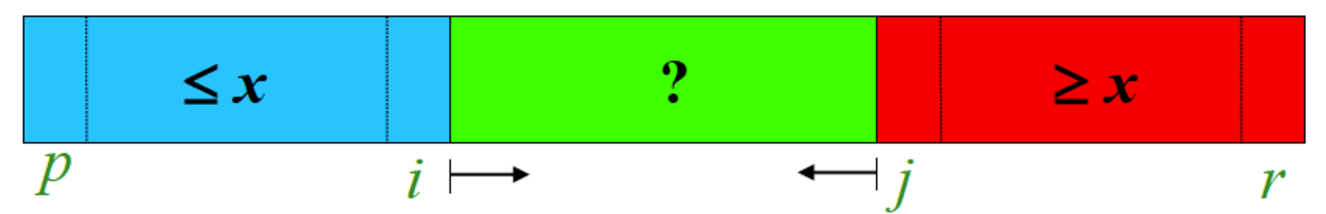
\includegraphics[scale=0.4]{imagenes/Hoare.png}
    \end{figure}
    
    \item ¿Qué ventajas y desventajas tiene elegir un pivote al azar?
    
    \item Una opción para elegir el pivote es: tomar el primer elemento, el del centro y el último, calcular la mediana entre los tres y elegir ese como pivote. Implemente esto en su código.

\end{enumerate} 

\problem \ptitle{Envoltura Convexa}

Dado un conjunto de $N$ puntos $P = \{(x_{1}, y_{1}), (x_{2}, y_{2}), \ldots, (x_{n}, y_{n})\}$ se define su \textbf{Envoltura Convexa} como el subconjunto de puntos $S \subseteq P$ con menos puntos tal que el polígono $P_{S}$ formado por los puntos en $S$ cumple que:
\begin{itemize}
    \item Es convexo
    \item Contiene a todos los puntos en $P$
\end{itemize}

\begin{center}
    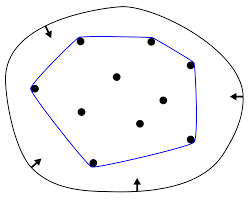
\includegraphics[scale=0.5]{imagenes/convexHull.png}
\end{center}    
El algoritmo de Graham para calcular la envoltura convexa es el siguiente:
\begin{enumerate}[1.]
    \item Encontrar el punto $p^*$ de menor coordenada $y$ (si hay más de uno elegir el de menor coordenada $x$)
    \item Ordenar los demás puntos respecto al ángulo formado con $p^*$
    \item Recorrer los puntos en orden creciente de ángulo y
    \begin{itemize}
        \item Agregarlo a la envoltura convexa si la línea formada con el siguiente punto es un giro derecha respecto a la línea anterior\\
        \item Sacarlo de la envoltura convexa si la línea formada con el siguiente punto es un giro izquierda respecto a la línea anterior y revisar el punto anterior.\\
        \begin{center}
        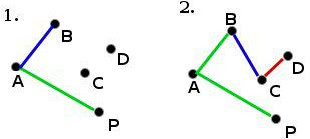
\includegraphics[scale=0.5]{imagenes/result.jpg}
        \end{center}
    \end{itemize}
\end{enumerate}
\begin{enumerate}
    \item Muestre que el punto 3. toma tiempo $\mathcal{O}(n)$, por lo que el algoritmo toma tiempo $\mathcal{O}(n\log n)$.
    \item Escriba la clase Punto que represente un punto en el plano. Además escriba dos Comparadores de puntos, uno que lo haga según su coordenada $y$ y otro que lo haga según el ángulo formado respecto a un punto $p$.
    \item Escriba la función \texttt{static Punto[] grahamScan(Punto[] P)}, que toma como entrada el conjunto de puntos $P$ y retorna su envoltura convexa, calculada según el algoritmo de Graham descrito anteriormente.
\end{enumerate}
\end{problems}
\end{document}